\section{Auswertung}
\label{sec:Auswertung}


\subsection{Blockschaltbild}
\subsection{Grafische Darstellung der Stackspannung, der
Stackleistung, der Verbraucherleistung und des Wasserstoffverbrauchs}
\begin{figure}[H]
    \centering
    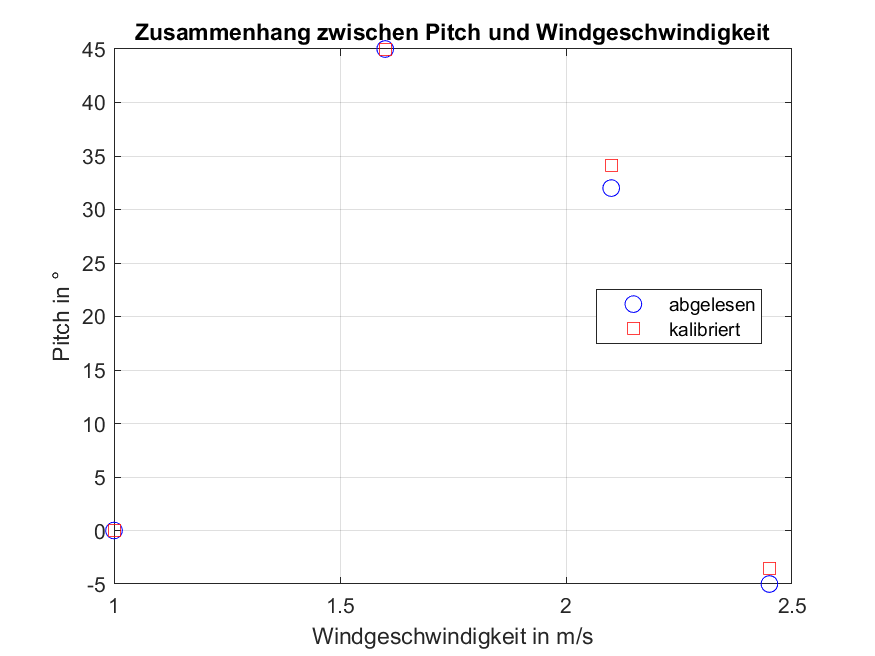
\includegraphics[width=0.8\textwidth]{plot1}
    \caption{Grafische Darstellung der Stackspannung, der
    Stackleistung, der Verbraucherleistung und des Wasserstoffverbrauchs.}
    \label{fig:plot1_26062023}
  \end{figure}
\subsection{Grafische Darstellung einiger Messgrößen im Bezug zum Verbracuherstrom}
\begin{figure}[H]
    \centering
    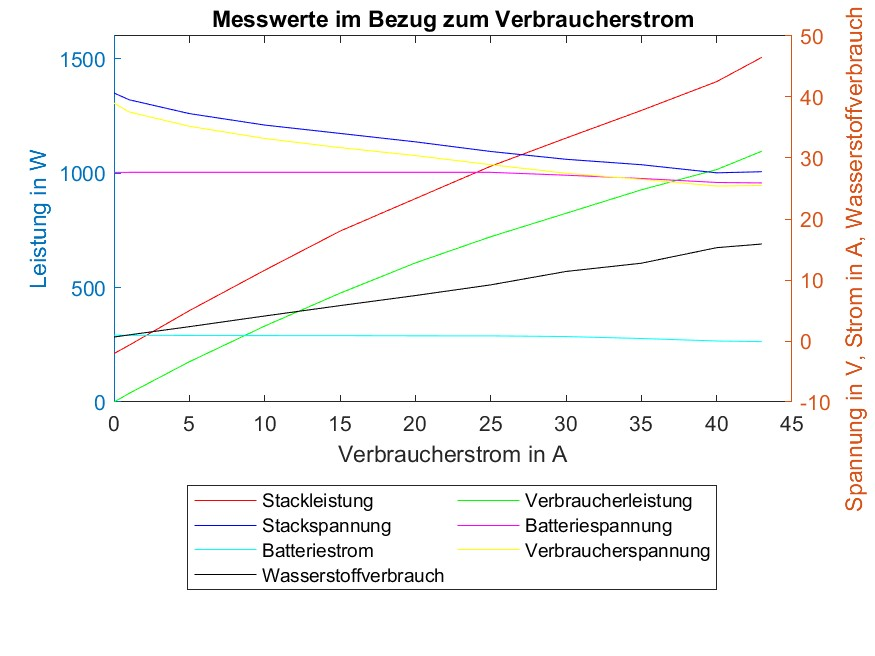
\includegraphics[width=0.8\textwidth]{grafik2}
    \caption{Grafische Darstellung der Stackspannung, der
    Stackleistung, der Verbraucherleistung und des Wasserstoffverbrauchs.}
    \label{fig:plot2_26062023}
  \end{figure}
  \begin{figure}[H]
    \centering
    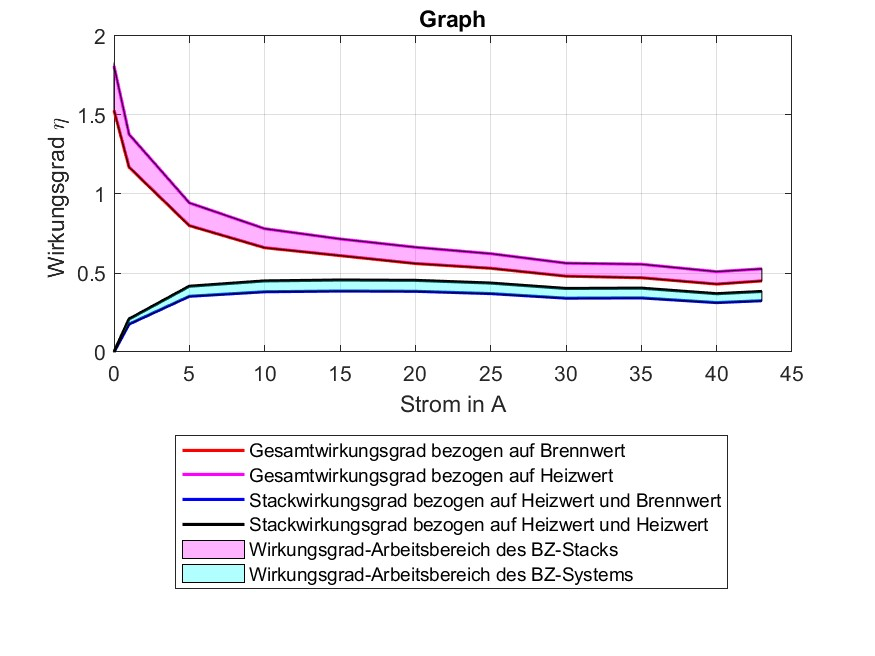
\includegraphics[width=0.8\textwidth]{plot3}
    \caption{Wirkungsgradverlauf für den Stack und das gesamte System.}
    \label{fig:plot3_26062023}
  \end{figure}
\subsection{Diskussion der Kurven}
\autoref{fig:plot1_26062023} und \autoref{fig:plot2_26062023} zeigt die unterschiedlichen Systemspannungen in Abhängigkeit des
Verbraucherstroms. Zu erkennen ist die charakteristische Brennstoffzellen Spannungskennlinie (hier
blau), die in \autoref{fig:plot2_26062023} genauer beschrieben wird. Die Stack- als auch die Verbraucherleistung
steigen in Abhängigkeit des zugeführten Wasserstoffes proportional an. In den \autoref{fig:plot1_26062023} und \autoref{fig:plot2_26062023} ist weiterhin zu erkennen, dass bei einem Verbraucherstrom ab ca. 40 A, sowohl die Stack- als
auch die Verbraucherspannung leicht, absinken. Die lässt sich auch an dem Abfallen des
Wirkungsgrades ablesen.
\subsection{}
\subsection{Teillastverhalten}

Leistung prinzipiell mit höherer Temperatur größer, außerdem Batteriestrom höher? 
Steigt der Teillastwirkungsgrad mit steigender Temperatur (nicht über betriebstemperatur) oder ist das unsinnig?
Warum ist der Batteriestrom auf einmal so hoch? Puffert die Batterie die Leistung aus die nicht mehr von der BZ bereitgestellt werden kann durch die höhere temperatur?



\subsection{Energiebilanz für den Teillastfall}